\chapter{Introduction}

\section{Description and specification}
It is required to analyze a multi-core computer equipped with \( N \) CPUs, which execute multiple interactive processes. The processes are dynamically generated at intervals of \( T \) seconds. Each process has a total duration \( D \), which is divided into three distinct execution phases:
\begin{enumerate}
    \item initial processing phase;
    \item I/O operation phase;
    \item final processing phase.
\end{enumerate}

The times \( T \) and \( D \) are defined as IID random variables. The processes are categorized into two types and generated as \textit{CPU bound} with probability \( p \) or \textit{I/O bound} with probability \( 1 - p \). The difference is that:
\begin{itemize}
    \item in CPU-bound processes the I/O operation phase constitutes 20\% of the total duration \( D \), and the other two phases both the 40\%;
    \item in I/O-bound processes the I/O operation phase constitutes 80\% of their total duration \( D \), and the other two phases both the 10\%;
\end{itemize}

Processes are assigned to CPUs by the operating system’s scheduler, which selects tasks from a list of “ready” processes. When a CPU becomes idle for entering the I/O operation phase or ending the final processing phase of a process, the scheduler immediately assigns it to a new ready process, if present. Once a process completes its I/O operation phase, it is marked as ready again and is returned to the scheduling queue. A process exits the system once it has successfully completed all three phases of execution.

The scheduler can be implemented to follow two distinct policies:
\begin{itemize}
    \item First Come First Served (FCFS): processes are scheduled in the order of their arrival after the generation or after the end of the I/O phase;
    \item Shortest Job First (SJF): scheduling is determined based on the shortest remaining time until either the process’s I/O phase or its completion.
\end{itemize}

\section{Objectives}

The aim of this project is to assess and analyze the execution of a multi-core scheduling system under varying operational scenarios. The objective is to determine the optimal characteristics of the systems to make it work without the need to discard processes. Furthermore, the analysis aims to assess the conditions under which the best system behavior is achieved in terms of resource use efficiency and time performance evaluation. In particular, the different configurations taken into consideration are the scheduling policies, the number of CPUs in the system, the type of the processes (CPU bound or I/O bound), the generation intervals and the duration of processes.

The overarching goal is to generate insights into optimal scheduling strategies and resource allocation practices for multi-core environments, enhancing system throughput and minimizing delays.


\section{Indices}

To evaluate the system’s performance comprehensively, the following indices will be analyzed in detail:
\begin{itemize}
    \item turnaround time $R$: defined as the total time elapsed from the arrival of a process in the system to its completion. This metric provides a measure of the computer’s overall responsiveness and of the time required for different types of processes to be executed;
    \item waiting time $W$: the cumulative time \cboh{COME LO CALCOLIAMO?} a process spends in the ready queue before being assigned to a CPU for execution. This metric represents the impact on the turnaround time of the queuing policy and of the workload of the system;
    \item CPU utilization of the $n_{th}$ CPU $\rho_n$: the fraction of time that each CPU is actively engaged in executing processes instead of being idle. This metric reflects the efficiency of resource usage within the system;
    \item active CPUs over time $N_A$: a dynamic measure of the number of CPUs actively processing tasks at any given moment. This index helps assess load distribution and system evolution;
    \item queue length over time $N_q$: tracks the size of the ready queue throughout the simulation, highlighting bottlenecks and variations in process scheduling.
\end{itemize}

These indices will be statistically analyzed to identify trends, anomalies, edge cases and key factors influencing system performance. By examining these metrics under diverse configurations of \( N \), \( p \) and scheduler policies, the project aims to provide actionable recommendations for improving the efficiency and adaptability of multi-core scheduling systems.

\section{Assumptions?}
To perform the analysis, the following assumptions are made:
\begin{itemize}
    \item There is sufficient memory to store the list of processes ready for execution, so the ready queue will be considered as infinite.
    \item The scheduler itself has a negligible load on the CPUs; there is no delay between the executions of the modeled processes. \cboh{assumiamo che sia zero? if not, quanto facciamo?}
    \item With the shortest job first (SJF) scheduling, an accurate estimate of the execution times is known a priori. If the scheduler is FCFS, this data is not used.
\end{itemize}




\section{Preliminary stability estimation}

The system can be modeled as a queueing network as shown in \autoref{fig:schema}.

\begin{figure}[H]
    \captionsetup{type=figure}
    \centering
    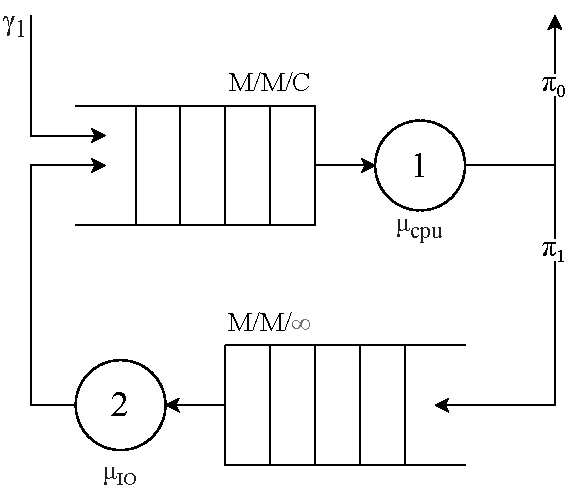
\includegraphics[width=0.6\textwidth]{images/03/schema.pdf}
    \captionof{figure}{Model of the system as a queueing network}
    \label{fig:schema}
\end{figure}

Let's analyze the system when the process generation time $T$ and the process duration $D$ are exponentially distributed, with mean values $E[T]$ and $E[D]$ respectively, and when the queues follow a FCFS scheduling policy.
New processes are generated at rate $\gamma_1=\frac{1}{E[T]}$.
The initial processing phase and the final processing phase are modeled by the $M/M/C$ Service Center $1$, where $C=N$ is the number of CPUs. 
Here it is assumed that the service time $t_{cpu}$ can be $0.4D$ for CPU bound jobs and $0.1D$ for I/O bound jobs. This means that, for total probability theorem, the mean value of the service time of the CPU processing is 
\[
E[t_{cpu}]=0.4 E[D] \cdot p+0.1E[D]\cdot (1-p) = 0.3E[D]\cdot p+0.1E[D]
\]
so that 
\[
\mu_{cpu}=\frac{1}{E[t_{cpu}]}=\frac{1}{0.3E[D]\cdot p+0.1E[D]}
\]
After the CPU processing phase, we can assume that it is equally likely that the process is at the beginning of the I/O phase or at the end of final processing phase. In the second case, it leaves the system with routing probability $\pi_0=\frac{1}{2}$.
If the process starts the I/O phase, it is routed with probability $\pi_1=\frac{1}{2}$ to the $M/M/\infty$ Delay Center $2$ with service time $t_{IO}$. 
Reasoning as before, the mean value of the service time of the I/O processing is $0.2D$ for CPU bound jobs and $0.8D$ for I/O bound jobs. The mean value of the service time of the I/O processing phase is
\[
E[t_{IO}]=0.2E[D]\cdot p+0.8E[D]\cdot (1-p)=0.8E[D]-0.6E[D]\cdot p
\]
so that
\[
\mu_{IO}=\frac{1}{E[t_{IO}]}=\frac{1}{0.8E[D]-0.6E[D]\cdot p}
\]

Both service centers are of type $M/M/C$, the external arrival $\gamma_1$ is Poissonian, routing probabilities are state-independent and arcs are traversed in zero time.
Therefore the hypothesis of Jackson's theorem are satisfied and the system admits a product form if the stabiity conditions $\rho_i=\frac{\lambda_i}{C_i\cdot \mu_i}<1$ are satisfied for each service center $i$.
To compute $\lambda_1$ and $\lambda_2$ we can define the routing matrix $\Pi=\begin{bsmallmatrix} 0 & \frac{1}{2} \\ 1 & 0 \end{bsmallmatrix}$. Arrivals are $\gamma=\begin{bsmallmatrix} \gamma_1 \\ 0 \end{bsmallmatrix}$.
It is $\lambda=(I-\Pi^T)^{-1}\cdot \gamma$. We can observe that, since the input and output must balance, $\gamma_1=\frac{\lambda_1}{2}$ and from the routing we get $\lambda_2=\frac{\lambda_1}{2}$. At the end we get $\lambda_2=\gamma_1=\frac{1}{E[T]}$ and $\lambda_1=\frac{2}{E[T]}$.

The stability condition for the delay center is always true, so the system is stable if the first service center is stable.
To have $\rho_1<1$ we get $\frac{\lambda_1}{N\cdot \mu_{cpu}}<1$: substituting and rearranging we get
\begin{equation}
    N > \frac{3p+1}{5}\cdot \frac{E[D]}{E[T]} 
\end{equation}

The metrics to be computed can be obtained from the analysis of the two
service centers. The mean number of busy CPUs is, for example,
\begin{equation}
    E[N_{cpu}]=\frac{\lambda_1}{\mu_{cpu}}=\frac{3p+1}{5}\cdot \frac{E[D]}{E[T]}
\end{equation}

And, with some computation based on known formulas, it is possible to get a theoretical estimation of
the mean number of processes in the ready queue $E[N_q]=E[N_{q_1}]$, of the mean
waiting time in the ready queue $E[W] = 2E[W_1]$ and of the turnaround
time $E[R] = E[W]+E[D]$.